\chapter{Úvod}

Celý svět kolem nás používá počítačové technologie s naprogramovanými aplikacemi. Právě kvůli tomu se s programováním setkáváme každý den, aniž bychom o tom věděli. Jedná se opravdu o užitečnou schopnost, kterou chceme rozvíjet. Samozřejmě je nejlepší začít v raném věku a to u dětí ve školním období. Je rozumné, když se malé děti setkají s programováním co nejdříve. Nejedná se pouze o schopnost umět naprogramovat aplikaci, ale především zapojení a trénování logického myšlení. Nejlepším způsobem jak se těmto schopnostem naučit je jednoznačně formou hry. V dnešní době existují hry, jako LightBot, Kodable a mnoho dalších, které děti rozvíjejí právě ve zmíněných okruzích. Často se jedná o hry, které jsou na menší zařízení, jako tablety, či telefony a dítě prochází hrou pouze za pomocí dotykové obrazovky. Dětem obecně pomáhá, když můžou při učení se nové věci manipulovat s fyzickým předmětem, protože zapojují více smyslů a díky kontaktu a prožitku se učí nové věci více kvalitně a v kratším časovém intervalu. My jsme chtěli do této problematiky také přispět, a proto jsme vymysleli a poté vytvořili hru s názvem Codeventure. Celkový návrh hry je navržený tak, abychom dokázali děti co nejefektivněji naučit zapojit logické myšlení a rozvinuli jejich schopnost základů programování. Hráč pro průchod hrou využívá fyzické kartičky, které představují jednotlivé herní kroky kvůli lepšímu učení. Pro nejlepší herní prožitek je vhodné si hru zapnout na velké zobrazovací ploše a využívat mobilní aplikaci pouze jako ovladač, který slouží pro přepínání a plnění jednotlivých herních úrovní. Hra využívá také umělou inteligenci, která rozpoznává jednotlivé kartičky naskenované hráčem po složení herní sekvence. Díky hře Codeventure dítě zažije nezapomenutelný zážitek, při kterém se naučí využívat logické myšlení, základy programování a ještě se přitom zabavý v kouzelném světě Codeventure, který čeká opravdu na kohokoliv.
\chapter{Teoretická část}

\section{Pojmy}

\subsection{WebSocket}

\subsection{Frontend}

\subsection{Backend}

\subsection{Kompilace}

\subsection{Kontejner}
A container is a standard unit of software that packages up code and all its dependencies so the application runs quickly and reliably from one computing environment to another. \cite{Kontejner}

\subsection{Framework}

\subsection{Komponenta}
Komponenta je menší část aplikace, která poskytuje určitou funkcionalitu aplikace.

\subsection{Herní engine}

\subsection{Cloud}

\subsection{VPS}

\subsection{API}

\subsection{Škálování}

\subsection{JSON}

\subsection{Transpilace}

\subsection{Transakce}

\subsection{Cache}

\section{Technologie}

\subsection{Unity}
Unity je herní engine určený hlavně pro nováčky, ale i pro pokročilé programátory. Jako programovací jazyk Unity využívá C\# vyvýjený firmou Microsoft. Tento programovací jazyk je jednoduchý pro nováčky a je jedním z nejzsnažších programovacích jazyků v současnosti na naučení. \cite{Csharp} Dají se v něm vytvářet 2D i 3D aplikace. Výsledná hra je spustitelná na mnoha platformách, od počítačů až po mobilní zařízení.

\subsection{JavaScript}
JavaScript je moderní programovací jazyk využívající se jak na frontendu, ale i na backendu. Jazyk je tzv. interpretovaný jazyk, což znamená, že kód je spustitelný rovnou ze zdrojového kódu a není potřeba jej kompilovat.

\subsection{TypeScript}
TypeScript je nadstavbou JavaScriptu, která poskytuje typování kódu. Díky tomu je ve výsledné aplikaci méně chyb spojených s typy, protože jsou kontrolovány během vývoje a sestavování aplikace. Ve výsledku je kód transpilován zpět do JavaScriptu.
TODO domyslet

\subsection{React.js}
React.js je JavaScriptový framework pro vývoj uživatelské rozhraní neboli UI. Tvoří se s ním dynamické webové aplikace nebo mobilní aplikace. Vývojářem tohoto frameworku je firma Meta (dříve známá jako firma Facebook). UI je děleno na menší komponenty, které mají svoji funkcionalitu a dají se mezi sebou jednoduše zaměňovat. Díky tomu není například potřeba načíst celou stránku při přechodu na jinou stránku, ale stačí pouze zaměnit komponenty které se na stránce změnily (např hlavička a patička zůstávají stále načteny, ale obsah stránky se změní).

\subsection{Next.js}
Next.js je JavaScriptový framework stavící na frameworku React.js. Je vytvářen společností Vercel, která pod stejným názvem provozuje i vlastní Cloud. Tento framework usnadňuje vývojáři práci se stránkami a přidává nezpočet výhod nad použitím samothného Reactu.js. Hlavním lákadlem je takzvaný "Server Side Rendering" což znamená, že počáteční kód který, je poslán klientovi, je nejdříve vykreslen na serveru, pak je odeslán v neživé podobě klientovi a až po té, co je stránka načtena tak se z něj stává dynamická stránka pomocí React.js. Mezi další výhody patří například automatická optimalizace velikosti obrázků podle toho, jak velké je klient potřebuje, aby se nemusely posílat zbytečně velké a neoptimalizované obrázky.

\subsection{Node.js}
Node.js je backendové prostředí běžící na JavaScriptovém kódu. Výhodou oproti starším programovacím jazykům které běží na serveru např. PHP je, že aplikace neustále běží na pozadí. To umožňuje o dost jednoduší práci s časem (např. načasování určitých událostí neboli Cronjobů) nebo práci v reálném čase pomocí WebSocketů.

\subsection{GraphQL}
GraphQL je je jazyk pro API rozhraní sloužící pro jednoduchou komunikací mezi aplikací a serverem. Typy dotazů se dělí na 3 skupiny: Query: získání dat ze serveru, Mutation: změna dat na serveru a Subscription: zasílání dat v reálném čase pomocí WebSocketů.

\subsection{MongoDB}
MongoDB je dokumentová databáze, která je používaná na velké objemy dat. Data jsou zde ukládána do dokumentů ve formátu JSON. Databáze je jednoduše škálovatelná mezi více zařízeními v tak zvaném "Replica Setu" (data jsou kopírovaná mezi všemi zařízením, aby bylo možné při výpadku některého zařízení pokračovat dál v chodu aplikace). Replica set umožňuje i další pokročilé funkce jako například "transakce".

\subsection{Redis}
Redis je databáze fungující na principu klíč a hodnota. Pod nějakým klíčovým slovem si můžeme uložit hodnotu a následně si můžeme tuto hodnotu zobrazit po zadání tohoto klíče. Databáze funguje primárně v operační paměti počítače, takže funguje velmi rychle a je velmi efektivní. Největší využití je pro ukládání do cache aby byl zrychlen chod aplikace. Databáze také podporuje poslouchání na určitých hodnotách a v reálném čase posílání hodnot na poslouchající klienty. Tato funkcionalita je nejideálnější s technologií WebSocket, nebo ideálněji s GraphQL komponentou "Subscription". 

\subsection{Docker}

\subsection{Kubernetes}
Kubernetes, also known as K8s, is an open-source system for automating deployment, scaling, and management of containerized applications. \cite{Kubernetes}

\subsection{TensorFlow}
\chapter{Praktická část}
Hra Codeventure je o tom, aby zaujala uživatele formou hry, představila svět programování a logického myšlení.\par
Hráč se v této hře zapojuje do plnění úkolů, kterými prochází jednotlivými sekvencemi hry, získává odměny, které ho motivují ke splnění cílového úkolu.\par Jedná se o propojení mobilního zařízení, vetší zobrazovací plochy a kartiček s povely, které hráč využívá k průchodu hrou. Zapojením příkazových kartiček do hry využívá hráč i své kreativity k dosažení určeného cíle, protože ve hře můžeme nalézt úrovně, které mají otevřené řešení. Složitost úrovní se stupňuje přímo úměrně s postupem hrou.\par Při přenosu příkazů z kartiček do hry se používá umělá inteligence, která rozpoznává jednotlivé příkazy a ty následně přenáší hráči na cílové zařízení a poté vidí vyhodnocení zvoleného postupu. Uvede postavičku do pohybu, která při správném sestavení sekvence kartiček dostane postavičku do cílového bodu, nebo vyhodnotí sestavu povelů, jako chybnou.\par
V momentu správného sestavení příkazových kartiček hra otevírá hráčí další kolo a odmění ho.\par Pokud se jedná o nesprávnou sekvenci, tak hra hráče upozorní na chybné řešení a průchod hrou musí opakovat za použití jiné kombinace kartiček.\par Na konci správně vyřešené úrovně je hráč hodnocen i za nejefektivnější způsob průchodu hrou, aby měl motivaci se dále zlepšovat a rozvíjet své vnímání logických příkazů směřujících k co nejlepšímu výsledku.

\section{Realizace}
\subsection{Architektura}

Cílem práce je vytvořit komplexní aplikaci, která využívá zařízení s větší obrazovkou jako prostředí pro běh hry, tzv. frontend, a mobilní telefon jako oddělený ovládací prvek (kontrolér). \par
Z tohoto rozdělení úkolů pak vychází základní nároky na architekturu systému skládající se z kontrolérové části (mobilní aplikace), zobrazovacího frontendu (webová aplikace) a serverového backendu, který musí zastat většinu funkcionality – především tedy autentizaci uživatelských zařízení (frontend i kontrolér) a jejich spárování, komunikaci s nimi, analýzu zaslaného obrazu, vykonávání analyzovaného uživatelského kódu a zprostředkování výsledků pro frontend. Samozřejmými součástmi a podsystémy jsou pak databázová část, emailová komunikace či cachování (využívání dočasné vyrovnávací paměti). Architekturu názorně shrnuje schéma na obr. \ref{fig:architektura}

\begin{figure}[h]
    \centering
    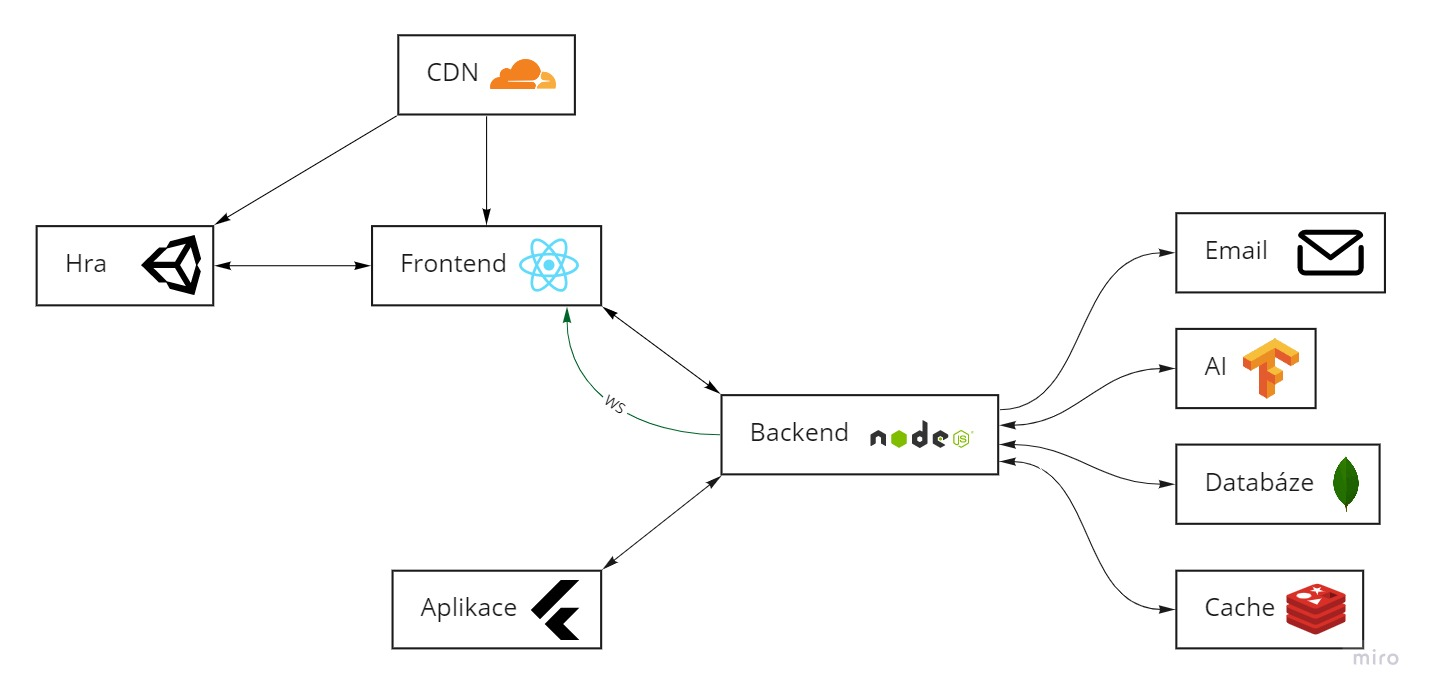
\includegraphics[width=0.6\textwidth]{img/architektura.jpg}
    \caption{Architektura aplikace.}
    \label{fig:architektura}
\end{figure}
\subsection{Backend}

\subsubsection{Využité technologie}
Jako stavební kámen pro backendovou část je použit Node.js s frameworkem Express.js. Na samotném Expressu běží GraphQL, které se stará o dotazy. Dále je zde také zaregistrován zpracovatel dotazů pro GraphQL Subscription, který zodpovídá za komunikaci v reálném čase.\par
Při použití jednoho serveru by bylo možné provozovat GraphQL Subscription pouze pomocí paměti tohoto jednoho serveru. Pokud bychom však chtěli rozdělit zátěž mezi více serverů, hrozilo by riziko, že dojde k desynchronizaci stavu kontrolérové části a frontendové části (například: Frontend si vytvořil komunikaci mezi sebou a serverem číslo 1. Další dotaz z kontroléru přišel na server 2, server tomuto zařízení odpověděl zpět bez problému, ale nebyl schopen oznámit frontendu o tom, že se něco stalo, protože tyto 2 servery o sobě navzájem neví). Proto je potřeba využít funkci Redisu s názvem Pub/Sub\cite{PubSub}, která oznámí změnu stavu všem podřízeným serverům.\par
Jako databáze byla zvolena databáze MongoDB, a to kvůli možnosti zpracovávat velké množství dat. Pro propojení backendu a databáze byla použita Prisma. Na dotazy, které by se často opakovaly, by nebylo efektivní se stále dokola dotazovat databáze, proto se určité, často opakované dotazy ukládají do cache paměti Redis.\par

\subsubsection{Autorizace}
Pro přístup k většině dotazů je potřeba být přihlášen. Uživatelé se můžou registrovat pomocí GraphQL mutace \uv{register} a přihlašovat pomocí \uv{login}. Při registraci jsou uživateli zkontrolována vstupní data, je vytvořen dokument s hodnotami: \uv{email}, \uv{first name}, \uv{last name} a \uv{password} (heslo je zahashováno pomocí bcrypt\cite{bcrypt}). Po vytvoření je vygenerována session a následně vrácen hash s ukrytým ID této session a jménem uživatele. Přihlášení potom funguje velmi podobně jako registrace, ale místo vytváření nového uživatele je vyhledán uživatel se stejným emailem a přiložené heslo je zkontrolováno na základě hodnoty uložené v databázi.\par
K přístupu k dotazům, ke kterým je potřeba být přihlášen, je potřeba zaslat v hlavičce dotazu vlastnost s názvem \uv{authorization} s hodnotou \uv{Bearer TOKEN}.\par
Pokud se chce uživatel odhlásit, je třeba spustit mutaci \uv{logout}, která smaže aktuální session z databáze aby se s ním nebylo možné dálé hlásit.\par
Při ztrátě hesla je možné spustit mutaci \uv{sendResetPassword} s parametrem email. Pokud v databázi existuje účet se zadaným emailem, tak je na něj zaslán email s odkazem obsahující resetovací token. Pomocí GraphQL mutace \uv{resetPassword} je při přiložení tohoto tokenu do 10 minut možné heslo změnit.\par
%TODO Vysvětlit token?
Kvůli bezpečnosti je také nutné mít možnost uživatelský účet smazat. Pro účel smazání účtu slouží GraphQL mutace \uv{deleteAccount}, při které musí být uživatel přihlášen a musí zadat aktuální heslo. Při této akci se nenávratně mažou všechna uživatelská data.

\subsubsection{Ovládání hry}
Jako jádro pro komunikaci mezi telefonem a hrou slouží GraphQL subscription s názvem \uv{unityCommunication}. Jako argument je potřeba token s přihlášením, protože při navazování WebSocketu se nezasílá hlavička dotazu.\par
Pro získání ostrovů a úrovní slouží GraphQL query \uv{islands} a \uv{levels}. Obě tyto query obsahují číslo ostrovu/levelu, data pro samotnou hru nebo mobilní telefon a úroveň obsahuje navíc počet hvězd, pokud již hráč tento level hrál.\par
%TODO Vysvětlit části hry
K nastavení aktuálního ostrova nebo úrovně se používají GraphQL mutace \uv{setUnityIsland} a \uv{setUnityLevel}. Obě nic nevrací a slouží k zasílání příkazů pro hru v prohlížeči.\par
Když hra potřebuje načíst ostrovy, je potřeba spustit GraphQL mutaci \uv{getUnityIslands}. Tato mutace nic nevrátí, ale ihned posílá hráči pomocí GraphQL subscription data pro vykreslení.\par
Pro nastavení rycholosti přehrávání výsledné animace slouží Graphql mutace \uv{setSpeed}, pomocí které se dá nastavit rychlost v rozmezí mezi 1x až 10x.

\subsubsection{Přihlášení pomocí QR kódu}
Aby uživatel nemusel psát heslo na chytré televizi nebo na zařízení bez klávesnice, nabící server přihlášení pomocí QR kódu. První musí začít poslouchat zařízení, na kterém se chce uživatel přihlásit pomocí GraphQL subscription s názvem \uv{qrLogin}. Tato subscription přijímá jako argument řetězec, který je pak použit pro přihlášení. Potom lze z již přihlášeného zařízení sputit GraphQL mutaci \uv{qrLogin} s stejným argumentem jako u subscription.

\subsubsection{Vyhodnocování úrovně}
Ještě před zobrazením zadání je potřeba požádat server o čas začátku řešení, aby bylo možné na konci zjistit, jak dlouho hráči trvalo vyřešit úroveň. K tomuto účelu slouží GraphQL query \uv{getTime}.\par
Samotné vyhodnocování úrovní probíhá v několika krocích viz obrázek \ref{fig:proces-vyhodnocovani}. Tyto kroky jsou rozepsané v následujících podkapitolách.

\begin{figure}[h]
    \centering
    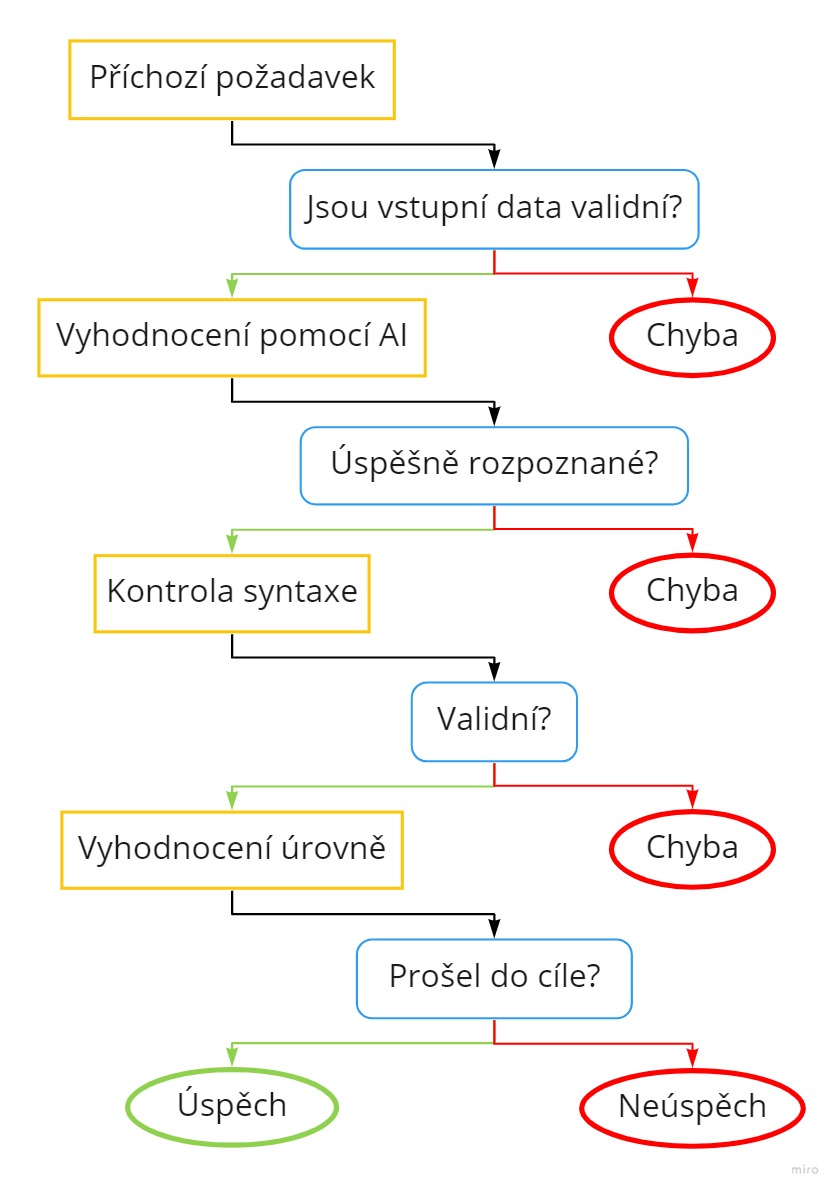
\includegraphics[width=0.3\textwidth]{img/proces.jpg}
    \caption{Proces vyhodnocování úrovně.}
    \label{fig:proces-vyhodnocovani}
\end{figure}

\subsubsubsection{Validace vstupů}
Před začátkem vyhodnocování je potřeba zkotrolovat, zda jsou všechny údaje validní. Backend pro tento krok očekává následující parametry: číslo ostrova a úrovně, čas ve kterém se začínalo řešit a fotografie kartiček. Pro zkontrolování integrity času je použit hash, kterému musí sedět kontrolní součet. Kdyby ho uživatel nějak změnil, nebyl by potom tento čas validní.

\subsubsubsection{Vyhodnocení pomocí AI}
Po zvalidování vstupů je potřeba vyhodnotit data na obrázku. Pro tento účel slouží samostatný vyhodnocovací backend, na kterém běží Express.js a TensorFlow.js. Na tomto backendu je uložen model vytrénovaný pomocí služby Microsoft Custom Vision. Tento backend není veřejně přístupný a komunikovat s ním může pouze hlavní backend.\par
Po přijetí obrázku jej hlavní backend zasílá pomocí API rozhraní backendu vyhodnocovacímu. Po úspěšném vyhodnocení jsou vráceny informace o tom, jak jsou kartičky průměrně velké, a pole s údaji, kde a s jakou přesností se konkrétní kartička nachází.

\subsubsubsection{Kontrola syntaxe a vyhodnocení úrovně}
Po vyhodnocení obrázku je provedena kontrola syntaxe a vyhodnocení úrovně.\par
Nejprve je potřeba zkontrolovat, zda rozpoznané kartičky obsahují \uv{Start} a \uv{Konec}. Dále je vypočítána přímka mezi dvěma body a jsou získány kartičky které na této přímce leží (pomocí průměrné velikosti kartiček si lze vypočítat toleranci od přímky). Pak jsou pomocí pravého úhlu dopočítány přímky pro tyto kartičky a jsou k nim přiřazeny rozšiřující kartičky.\par
Když se někde vyskytne synkatická chyba (chybí kartička \uv{Start} nebo \uv{Konec}, kartička je na místě, na kterém být nemůže), je hráči oznámeno, co udělal špatně a pokus je vyhodnocen jako neúspěšný.\par
Poslední částí je vyhodnocení úrovně. Pro tuto část je potřeba získat z databáze data o tom, jak úroveň vypadá. Server prochází úroveň krok po kroku a z toho zjišťuje, jak si hráč vede. Nakonec server odesílá data o výsledku zpět do kontroléru a na frontend, kde se hráč dozví celkové hodnocení.

\subsubsection{Nasazení na server}
Nasazení na server je klíčový krok, který určuje zda je celá hra hratelná.
% ??? Sem by měla nejprve přijít věta o tom, že je použit docker, do něj že patří komponenty, takže musíme vytvořit vlastní a pak popisovat co a jak.
Pro vytvoření vždy identického prostředí je potřeba vytvořit kontejner, který obsahuje pouze data potřebná k běhu služby.\par
Pro vytvoření kontejnerů je použit Docker. Pomocí takzvaného \uv{Dockerfile} je zadefinován postup jak backend sestavit, který když následně sestavíme, dostaneme balík, který je možné kdekoliv sputit. Tento proces je vykonán jak u hlavního backendu, ale i u vyhodnocovacího backendu.\par
K následnému nasazení na server je použita platform Kubernetes, konkrétně K3s, která se stará o kontejnery, zajišťuje síťovou komunikaci a rozprostřívá zátěž mezi servery.

\subsection{Web}
Web neboli frontend je hlavní částí, kterou uživatel vidí. Jeho úkoly jsou: zobrazení informací, správa uživatelského účtu a zobrazování hry. Klíčové prvky jsou rozepsané v~následujících podkapitolách.

\subsubsection{Prototyp}
Celkový Frontend webové aplikace je navržen a řádně otestován softwarem \uv{Figma}. Prvním krokem je vytvoření celkového vzhledu a designu aplikace. Rozhraní musí být co nejjednodušší a přehledné, jelikož je cíleno na mladší děti. Po navržení následovalo několik testů UX/UI. \uv{Figma} velice usnadní vývoj aplikace, protože jednotlivé části webu jsou navržené a celkové chování webu je nasimulované díky využitému prototypování, které \uv{Figma} nabízí. Z~návrhu vychází kompletní vzhled a fungování webové aplikace.

\subsubsection{Statická část}
Web je postaven na frameworku Next.js, který používá pro zobrazování React.js. Cílem bylo vytvořit web co nejrychlejší a nejspolehlivější.\par
Aby byl web co nejrychlejší, je potřeba, aby všechny části byly předem vygenerované a aby nebylo nuté zbytečně čekat při dotazu. Next.js v~základním stavu počítá s~tím, že obrázky jsou optimalizované při času jejich dotazu. Tato funkce je užitečná na stránkách s~proměnlivým obsahem, nikoliv na staticky generovaných stránkách. Proto jsme aplikovali trochu netradiční řešení, a to optimalizaci obrázků při generování webu. Díky tomu není potřeba žádný speciální server a je potřeba jen všechny soubory někam umístit.\par
Pro co nejrychlejší a nespolehlivější běh webu je potřeba umístit jej na takový server, který bude schopen rychle odpovídat velkému množství lidí. Pro tento účel byl vybrán hosting Cloudflare Pages\cite{Cloudflare-pages} s~jejich vlastní CDN\cite{Cloudflare-cdn}. 

\subsubsection{Správá účtu}
Důležitou částí webu je přihlašovací systém a následná správa účtu. Pro přihlášení je možné použít email a heslo (pomocí GraphQL mutace \uv{login}) nebo QR kód, který se dá naskenovat pomocí mobilní aplikace (GraphQL subscription \uv{qrLogin} a stejnojmenná GraphQL mutace). Dále je zde možnost zaregistrovat se (mutace \uv{register}) a resetovat heslo pomocí zaslání emailu (mutace \uv{sendResetPassword}).\par
Když je uživatel přihlášen, je možné odhlásit se (mutace \uv{logout}) nebo aktuální účet smazat (mutace \uv{deleteAccount}).

\subsubsection{Hra}
Hra je vytvořena pomocí herního enginu Unity. Aby bylo možné ji spustit v~prohlížeči, je zde použita možnost exportu do webového prostředí zvaná \uv{WebGL}.
Pro následnou integraci Unity do webového prostředí slouží knihovna \uv{react-unity-webgl}\cite{react-unity-webgl}, která poskytuje integraci kódu v~Unity s~kódem v~Reactu.

\subsubsubsection{Komunikace}
Klíčovou funkcí hry je komunikace mezi backendem a hrou tak, aby bylo možné zobrazovat úkony hráče. Tuto práci výrazně zlehčuje již zmíněná knihovna \uv{react-unity-webgl}\cite{react-unity-webgl}. Díky této knihovně není třeba komunikovat s~backendem dalším způsobem a je možné použít již existující spojení mezi frontendem a backendem.\par
Komunikace pak může probíhat oběma směry. Směr \uv{hra na backend} je použit pouze jednou, a to při načtení - když hra potřebuje vykreslit ostrovy. Této akce je docíleno pomocí připravené funkce v~Reactu, která prostřednictvím GraphQL mutace \uv{getUnityIslands} kontaktuje server, aby zaslal zpět nové ostrovy. Tuto funkci lze použít pomocí Unity metody \uv{GetIslands}.\par
Druhý směr komunikace je častější, a to \uv{backend na hru}. Pro tento směr je potřeba nejdříve navázat spojení pomocí GraphQL subscription \uv{unityCommunication}. Backend má pak možnost provést jakoukoliv veřejnou metodu umístěnou v~komunikačním skriptu. Jako argument může přiložit data, která chce předat. Tato data jsou ve formátu JSON a je třeba je po přijetí deserializovat. Používá se například pro přejetí kamery na jiný ostrov, nebo nastavení objektů do scény se zadáním.

\subsubsubsection{Načítání modelů}
Aby byla hra co nejmenší a aby se nenačítala velmi dlouho, je potřeba rozdělit hru do více částí a následně tyto části načítat podle potřeby hráče. Pro tento účel slouží balíčkový systém zvaný \uv{AssetBundle}\cite{AssetBundle}. V~následných balíčcích jsou obsaženy modely a animace k~jednotlivým ostrovům, které se načítají podle toho, co uživatel zvolí na kontroléru.

\subsubsubsection{Animace}
Poslední důležitou částí jsou animace. Animace jsou přidávány na modely pomocí koster. Díky tomu je možné použít jeden model s~více animacemi. Připojené animace jsou pak spouštěny pomocí koprogramů, které si navzájem předávají informace. 

\subsection{Mobilní aplikace}
Mobilní aplikace je největší část, se kterou uživatel interaguje. Uživatel přes tuto část ovládá veškeré chování hry (hru jinak nejde ovládat), vybírá úrovně a skenuje svoje řešení pomocí fotoaparátu. Naprogramovaná je pomocí programovacího jazyku Dart s frameworkem Flutter. 

\subsubsection{Autorizace}
Autorizace se jako u webu provádí pomocí GraphQL mutace \uv{login}. Tento token je pak uložen v úložišti telefonu zvaném \uv{SharedPreferences}\cite{SharedPreferences} nebo na zařízeních s iOS v \uv{NSUserDefaults}\cite{NSUserDefaults}. Pomocí tohoto tokenu je zařízení autentifikováno vůči serveru.

\subsubsection{Skenování}
Pro focení slouží knihovna \uv{image\_picker}\cite{ImagePicker}. Tato knihovna využívá hlavní aplikaci na focení od výrobce, díky čemuž mají fotografie vysokou kvalitu.\par
Nejdříve je potřeba, aby uživatel zvolil ostrov a úroveň. Po odstartování pokusu se uživateli otevírá aplikace s fotoaparátem a je potřeba vyfotit své řešení úrovně. Následovně je fotografie z kapacitních důvodů zmenšena. Takto zmenšená fotografie je zaslána na server s potřebnými parametry mutací \uv{levelResult}. Server tento dotaz během pár vteřin zpracuje a zasílá hráči celkové hodnocení.


\section{Bezpečnost}
Zabezpečení je důležitou částí každé webové aplikace. Kvůli rozlehlosti tohoto projektu je potřeba, aby byla každá část zabezpečená ve všech ohledech.\par
Nejvíce zranitelná část je část webová. Nejvýznamnější bezpečností rizika zaznamenává nadace OWASP\cite{OWASP} s jejich seznamem \uv{Top 10 Web Application Security Risks}\cite{OWASP-top-ten}. V seznamu je 10 nejčastějších bezpečnostích rizik, ktereeá byla v posledních letech nejfrekventovanější.\par
Backendová i frontendová část má většinu těchto chyb odlazených a neměly by být zneužitelné. Zde jsou konkrétní příklady některých bodů:
\begin{itemize}
	\item \textbf{Kryptografické selhání}\cite{CryptographicFailures}: Všechny části předpokládají komunikaci pomocí šifrovaného protokolu (HTTPS). Certifikáty jsou podepsané od kryptografických autorit - Let's Encrypt a Cloudflare. Hesla jsou v databázi hashovaná pomocí šifrovací funkce \uv{bcrypt}\cite{bcrypt}.
	\item \textbf{Injection}\cite{Injection}: Rozhraní GraphQL validuje integritu datových typů, při práci s textem je tento text zkontrolován pomocí knihovny \uv{validator}\cite{Validator} pro správný formát. ORM framework Prisma vytváří bezpečné dotazy, aby nebylo možné vytvořit NoSQL inject.
	\item \textbf{Zranitelné a zastaralé komponenty}\cite{VulnerableAndOutdatedComponents}: Všechny balíčky, které jsou použity, jsou z oficiálních zdrojů (NPM, pub.dev). Balíček musí splňovat alespoň jednu z těchto specifikací: je na dané platformě populární (vysoký počet stažení), má bezproblémový zdrojový kód (musí být manuálně prověřeno) nebo vlastní balíček. Bezproblémovost balíčků automaticky kontroluje GitHub Dependabot, který monitoruje použité balíčky a při výskytu problému vytváří automaticky opravy.
\end{itemize}


\section{3D Modely}
Každý model je složen ze tří základních složek, a to \uv{vertices}, \uv{edges} a \uv{faces}, které definují celkový tvar a vzhled. Pro tvorbu modelů do hry je využit \uv{Low Poly}\cite{LowPoly} styl, díky čemuž mají výsledné objekty menší počet polygonů a jsou více optimalizované. Pro tvorbu objektů byl využit software Blender, který je ideální volbou pro tvorbu 3D grafických podkladů pro hru. Herní modely jsou využity v Unity a mobilní aplikaci.

\subsection{Box modeling}
\uv{Box modeling}\cite{BoxModeling} je technika modelování, při které jsou využity pouze základní objekty (jako je krychle, koule, atd.). Tento objekt je následně použit k dosažení finálního tvaru objektu dle připraveného návrhu. Celkový cyklus je opakován s každým novým prvkem a jednotlivé modely jsou poté kombinovány k dosažení cílového tvaru.

\subsection{Low poly}
Pro tvorbu jednotlivých herních modelů je využit styl \uv{Low poly}\cite{LowPoly}, který nabízí vysokou optimalizaci pro herní využití. \uv{Low poly} modely vypadají jednoduché, přičemž představují zákaldní tvar představované věci.

\subsection{Jednotlivé herní modely}
Na začátku tvoření modelů bylo hlavní vybrat časoprostor, kam celou hru zasadit. Herní modely jsou vymodelovány v prostředí příběhu o magickém světě a kouzelníkovi, který zachraňuje svoji planetu.

\subsubsection{Postavy}
\paragraph{Hlavní postava}
Model hlavní postavy je klíčový, protože představuje hráče a jeho postup hrou doprovází na každém kroku. Jak můžeme vidět na obr. \ref{fig:hlavni-postava}, tak model kouzelníka je hravý a jednoduchý. K modelu je vytvořena také sada animací pro jednotlivé pohybové operace ve hře.

\begin{figure}[h]
    \centering
    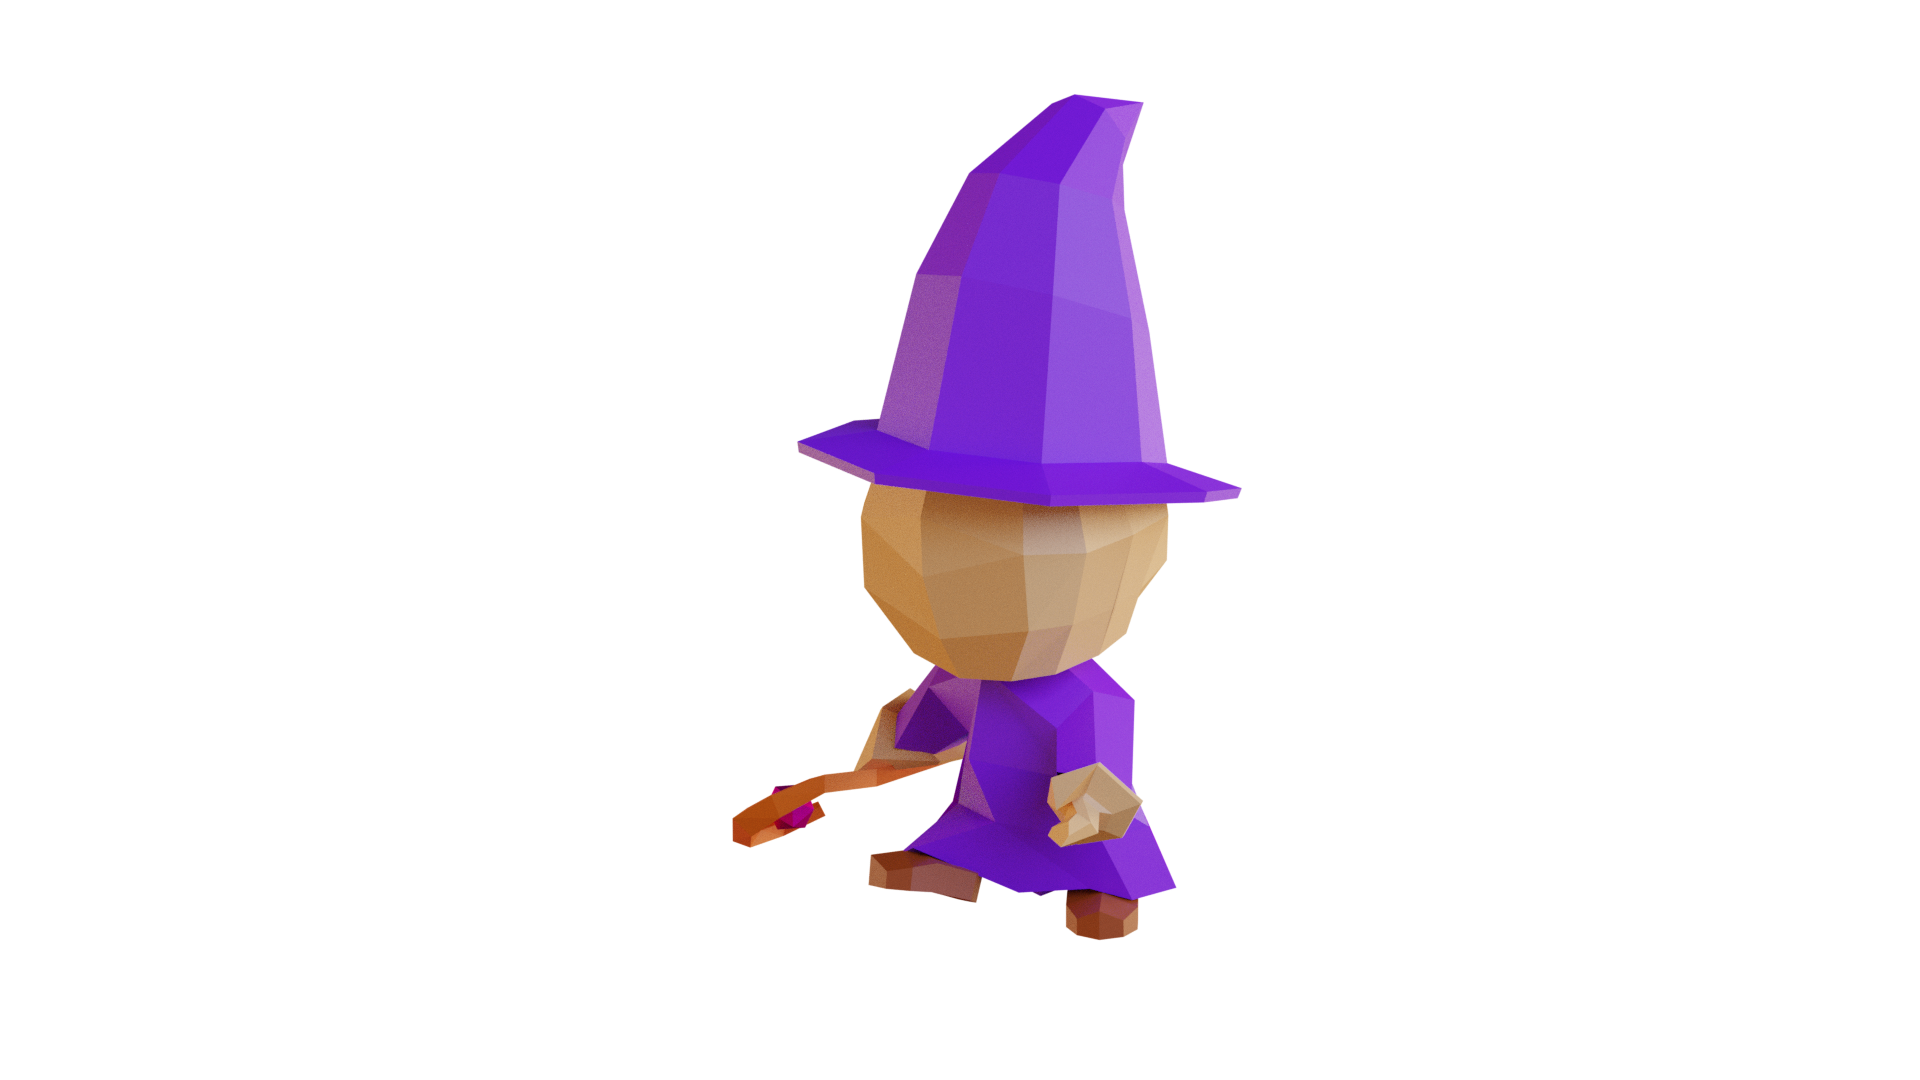
\includegraphics[width=0.6\textwidth]{img/hlavni-postava.png}
    \caption{Model hlavní postavy.}
    \label{fig:hlavni-postava}
\end{figure}

\paragraph{Nepřátelé}
Každý ostrov má sadu nepřátel, které hráč může nalézt v jednotlivých úrovních. Nepřátelé mají za úkol hráči ztížit průchod úrovní. Jednotlivé nepřátelské jednotky mají sadu animací. Modely nepřátel můžeme vidět na obr. \ref{fig:nepritel-golem}, nebo obr. \ref{fig:nepritel-cerv}.

\begin{figure}[h]
    \centering
    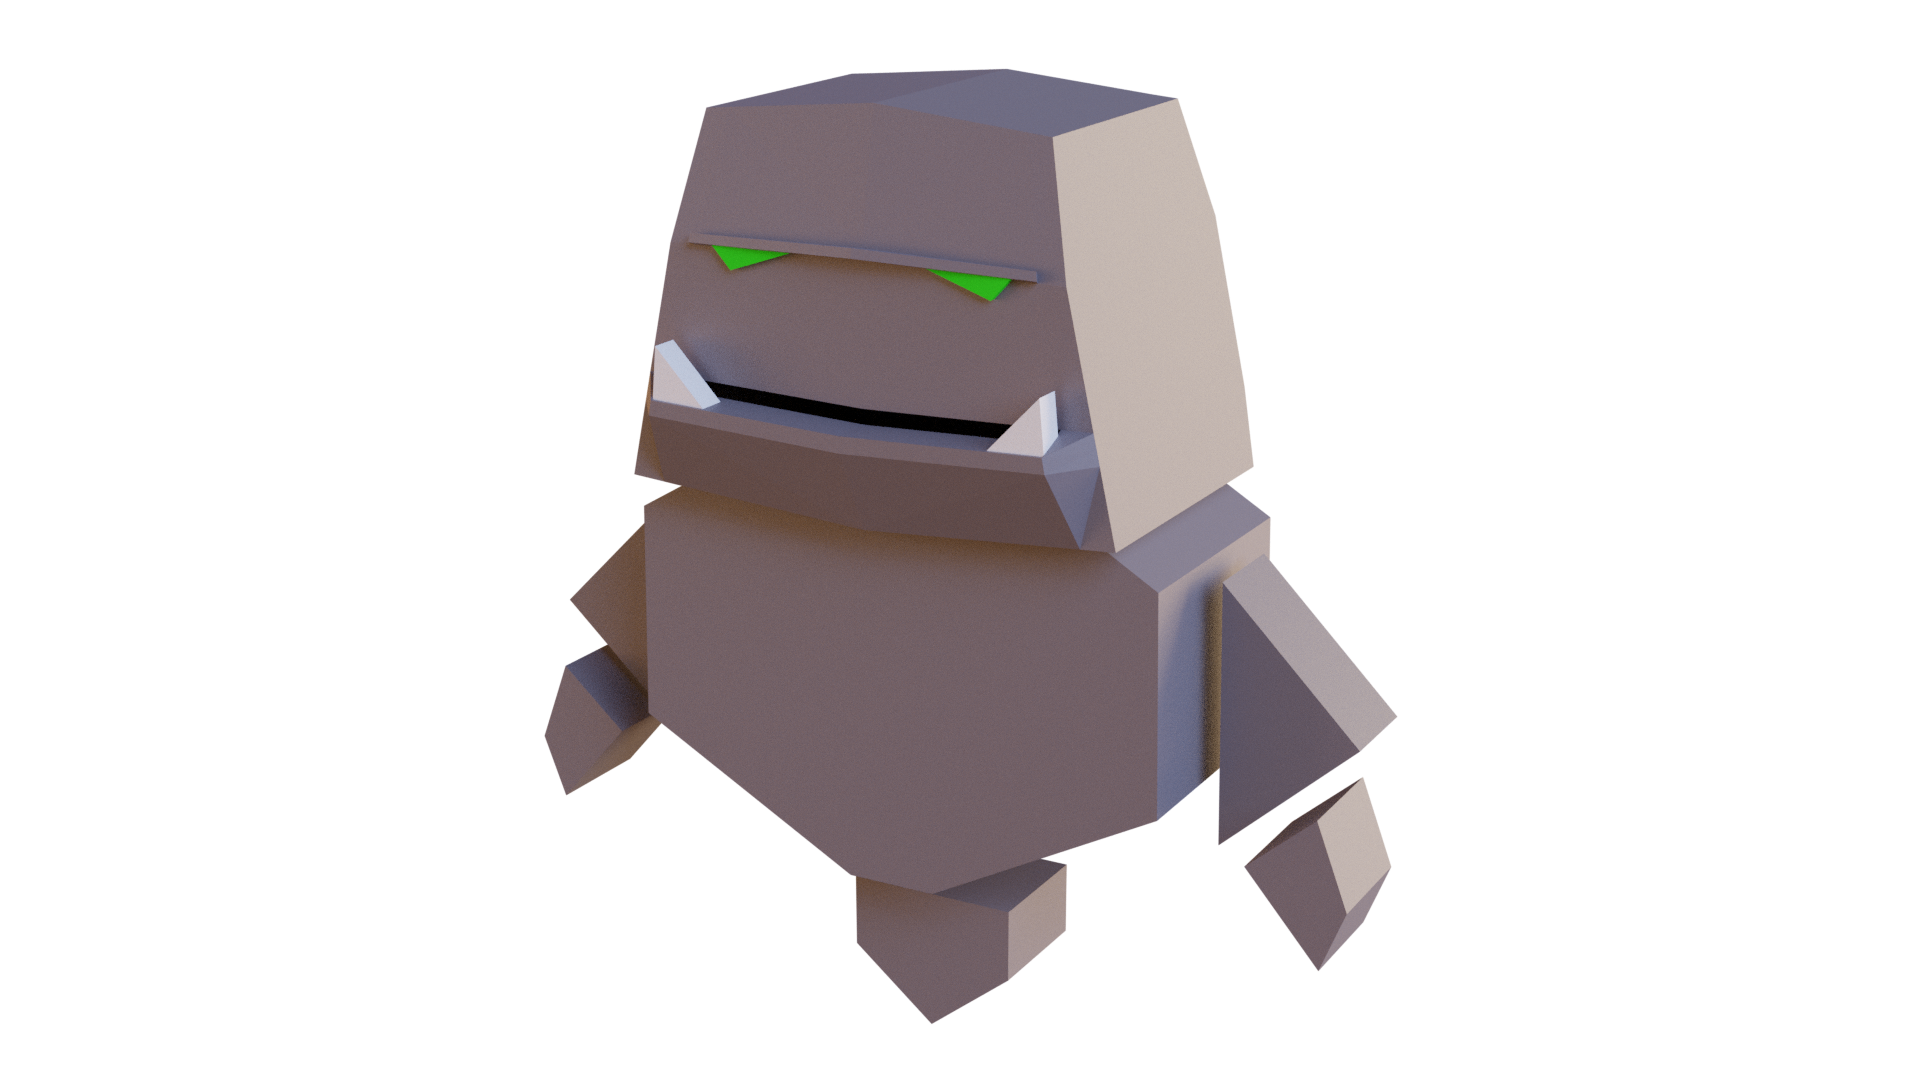
\includegraphics[width=0.6\textwidth]{img/nepritel-golem.png}
    \caption{Model nepřítele - Golem.}
    \label{fig:nepritel-golem}
\end{figure}

\begin{figure}[h]
    \centering
    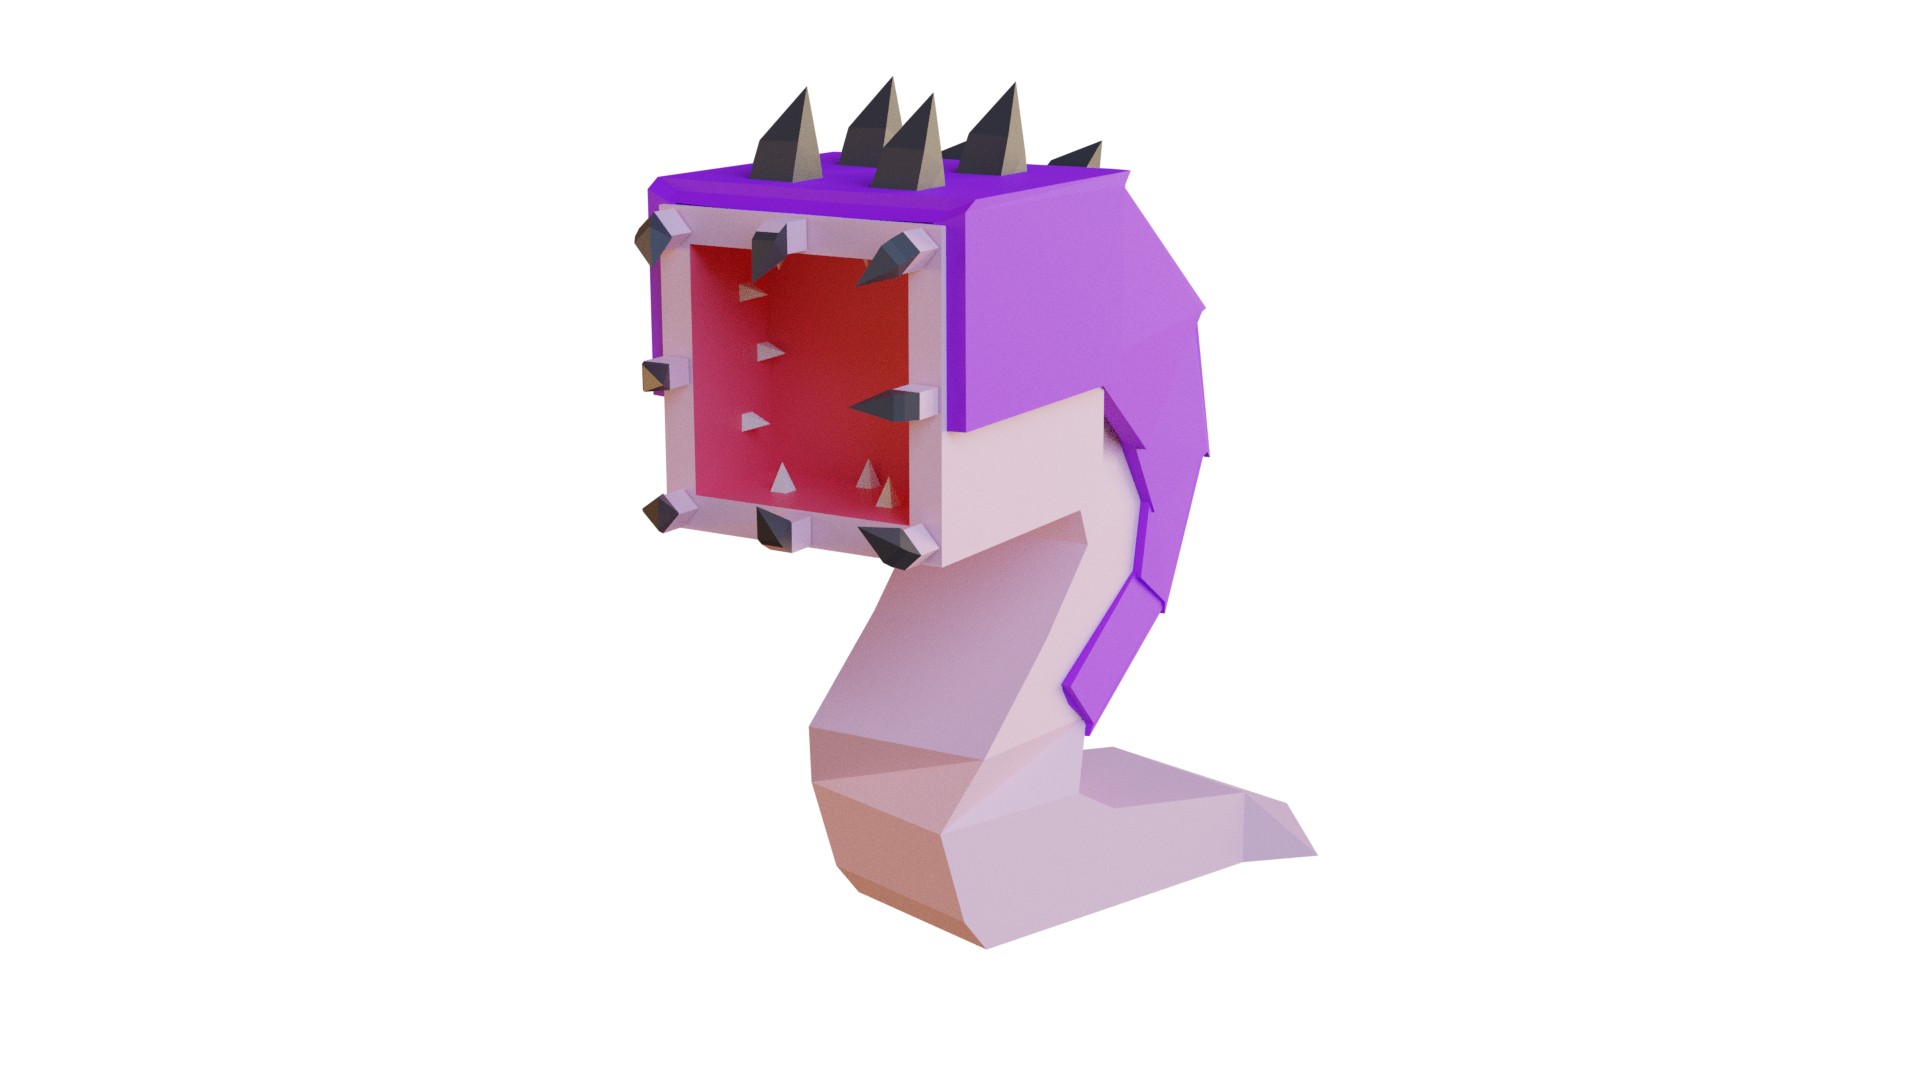
\includegraphics[width=0.6\textwidth]{img/nepritel-cerv.png}
    \caption{Model nepřítele - Červ.}
    \label{fig:nepritel-cerv}
\end{figure}

\subsubsection{Ostrovy}
Jednotlivé modely ostrovů představují přírodní elementy. Dle jednotlivých elementů jsou zbarvené a doplněné o modely, které jsou ve spojitosti s tímto elementem vyzobrazeny. Modely ostrovů jsou využity v mobilni aplikaci, jako je vidět na obr. \ref{fig:mobilni-aplikace-ostrov} Dominantou každého ostrova je krystal, který musí hráč získat pro úspěšné splnění. Ukázka zmiňovaného modelu obr. \ref{fig:nature-island}.

\begin{figure}[h]
    \centering
    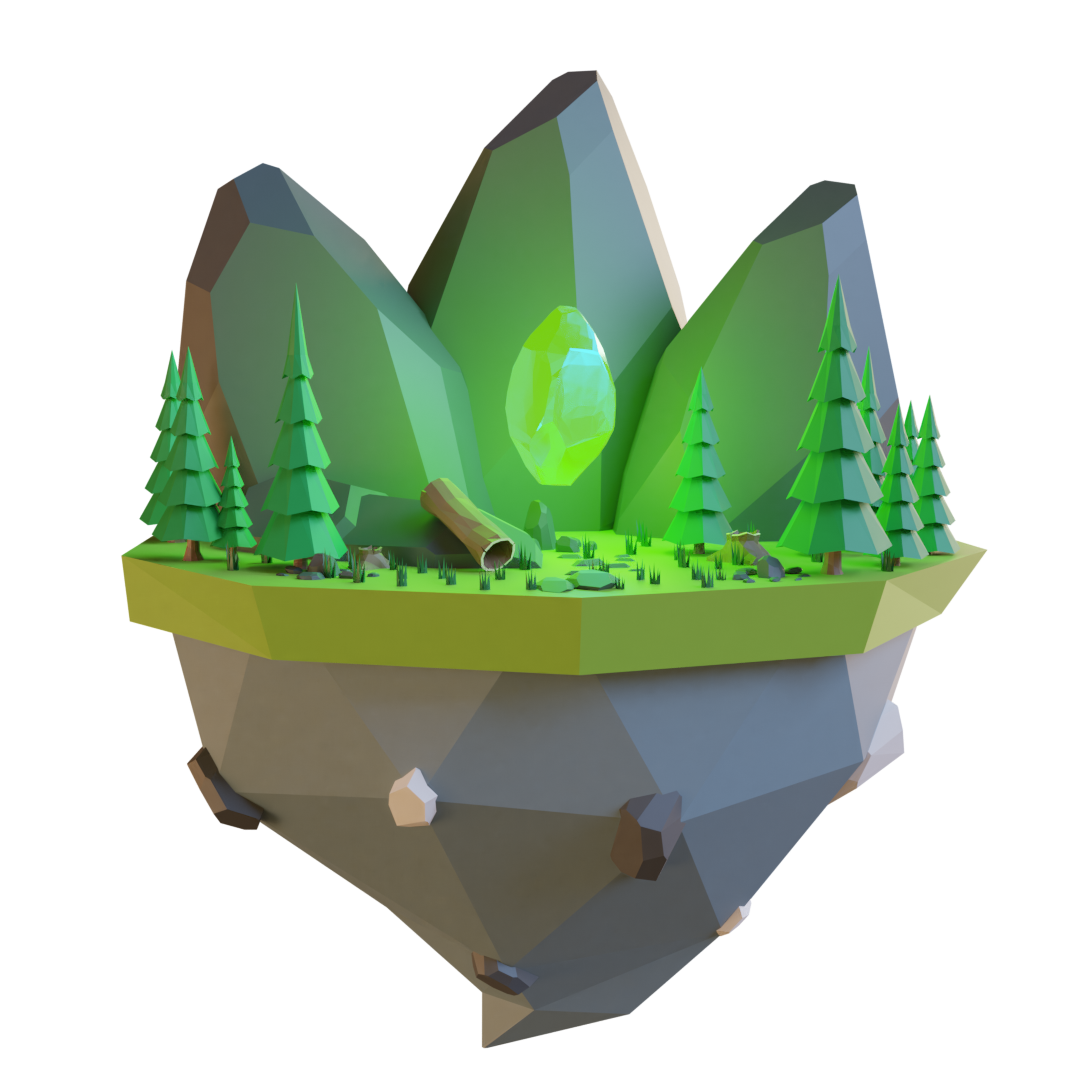
\includegraphics[width=0.6\textwidth]{img/NatureIsland.png}
    \caption{Model ostrova - Zemní ostrov.}
    \label{fig:nature-island}
\end{figure}

\begin{figure}[h]
    \centering
    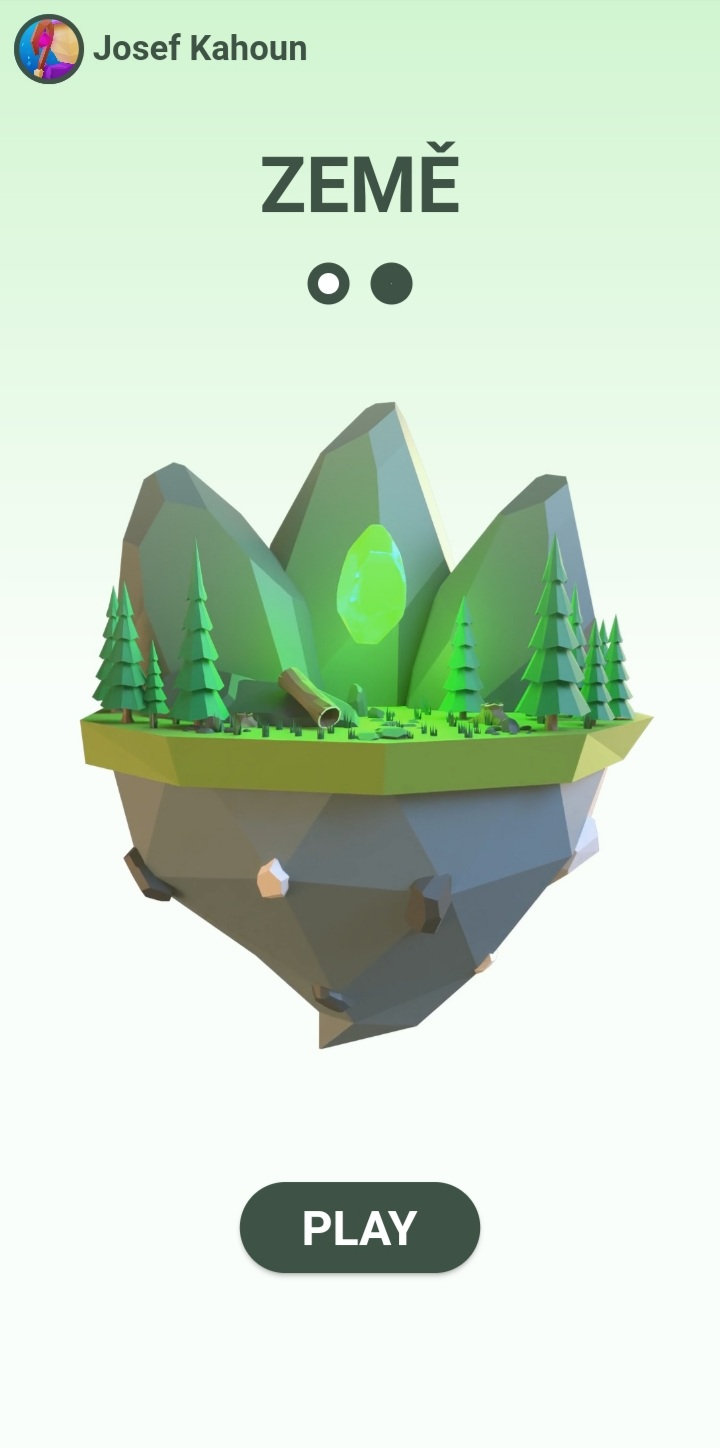
\includegraphics[width=0.6\textwidth]{img/mobilni-aplikace-ostrov.jpg}
    \caption{Model ostrova v mobilní aplikace.}
    \label{fig:mobilni-aplikace-ostrov}
\end{figure}

\subsubsubsection{Úrovně}
Jednotlivé úrovně tvoří mřížku, jako je vidět na obr. \ref{fig:model-levelu}. Každá úroveň představuje stejný element, jako je ostrov, ke kterému patří. Celá hra je odehrávána na herních plošinách. Jednotlivé plošiny, které jsou rozmístněny v mřížce úrovně, slouží jako umístitel, na kterém se můžou nacházet modely herních postav, bariér, cest, či ukazatelů cíle. Prostředí okolo herních plošin je doplněno o modely mateřského ostrova. Úkázka herního prostředí úrovně, je vidět na obr. \ref{fig:model-levelu}

\begin{figure}[h]
    \centering
    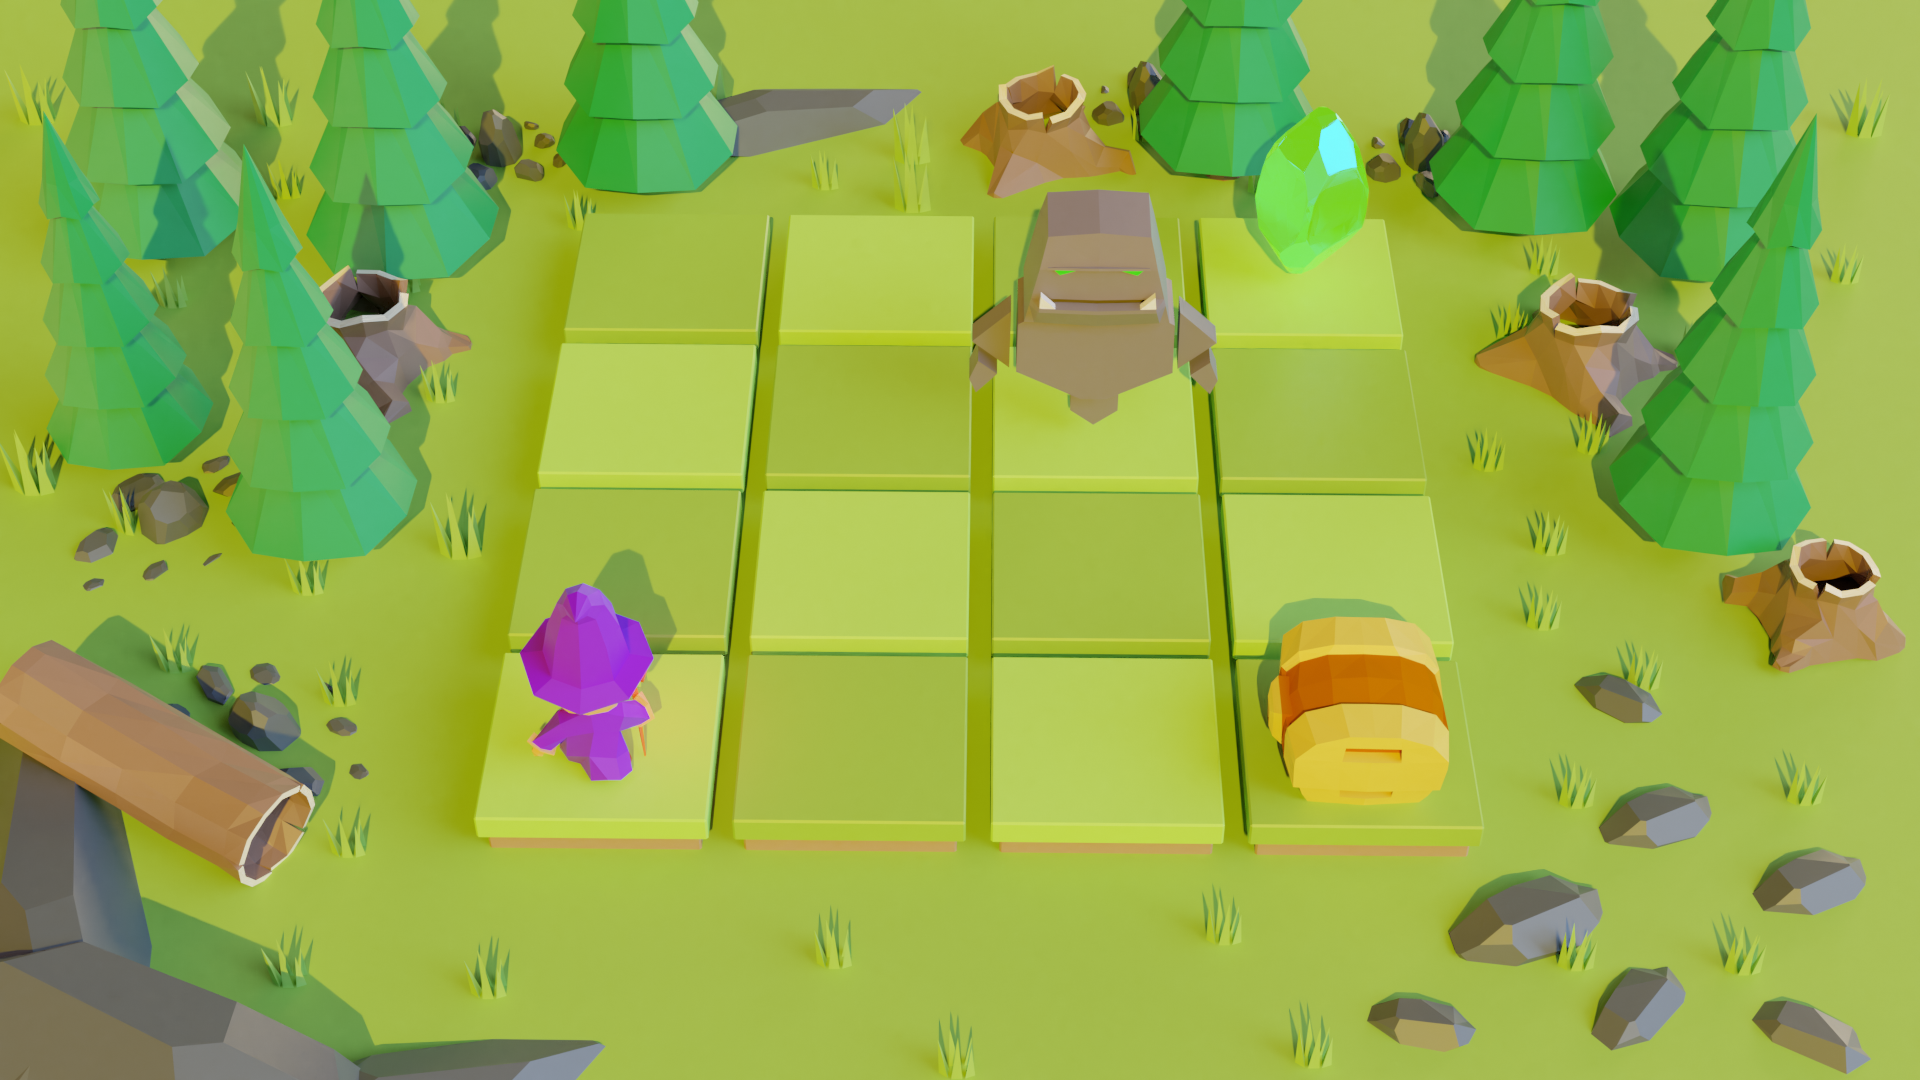
\includegraphics[width=0.6\textwidth]{img/model-levelu.png}
    \caption{Model úrovně.}
    \label{fig:model-levelu}
\end{figure}

\section{Popis hry}
Pro hraní hry je potřeba mobilní telefon s aplikací Codeventure, herní kartičky a zobrazovací zařízení, na kterém lze spustit webová aplikace. Nejlepší herní požitek hráč získá při velké ploše zobrazovacího zařízení. Prvním krokem je vytvoření herního účtu, kde se ukládá jednotlivý postup hráče hrou. Následuje stažení mobilní aplikace, kde se hráč přihlásí již vytvořeným účtem. Poté se přesune ve webové aplikaci do hry, kde uvidí první ostrov. Dále hráč využívá pouze mobilní telefon, a to jako ovladač. Na mobilím zařízení si zvolí ostrov a úroveň, kterou chce splnit. Před spuštěním levelu se hráči ukáže slovní zadání úkolu. Dalším krokem je vyobrazení herního zadání ve webové aplikaci a v mobilní spuštění fotoaparátu pro naskenování kartiček. Hráč musí pro úspěšné splnění úrovně seskládat validní a správnou sekvenci kartiček a poté ji naskenovat. Na obr. \ref{fig:pohled-hrace} můžeme vidět herní zadání a naskenovanou karetní sekvenci. Po vyhodnocení se hráči na mobilním telefonu zobrazí, jestli uspěl, či nikoliv. Jednotlivé úrovně může opakovat, nebo může zvolit jinou úroveň. Hra se snaží hráče nabádat k používání sofistikovanějších řešení a díky tomu jej posouvat. 

\begin{figure}[h]
    \centering
    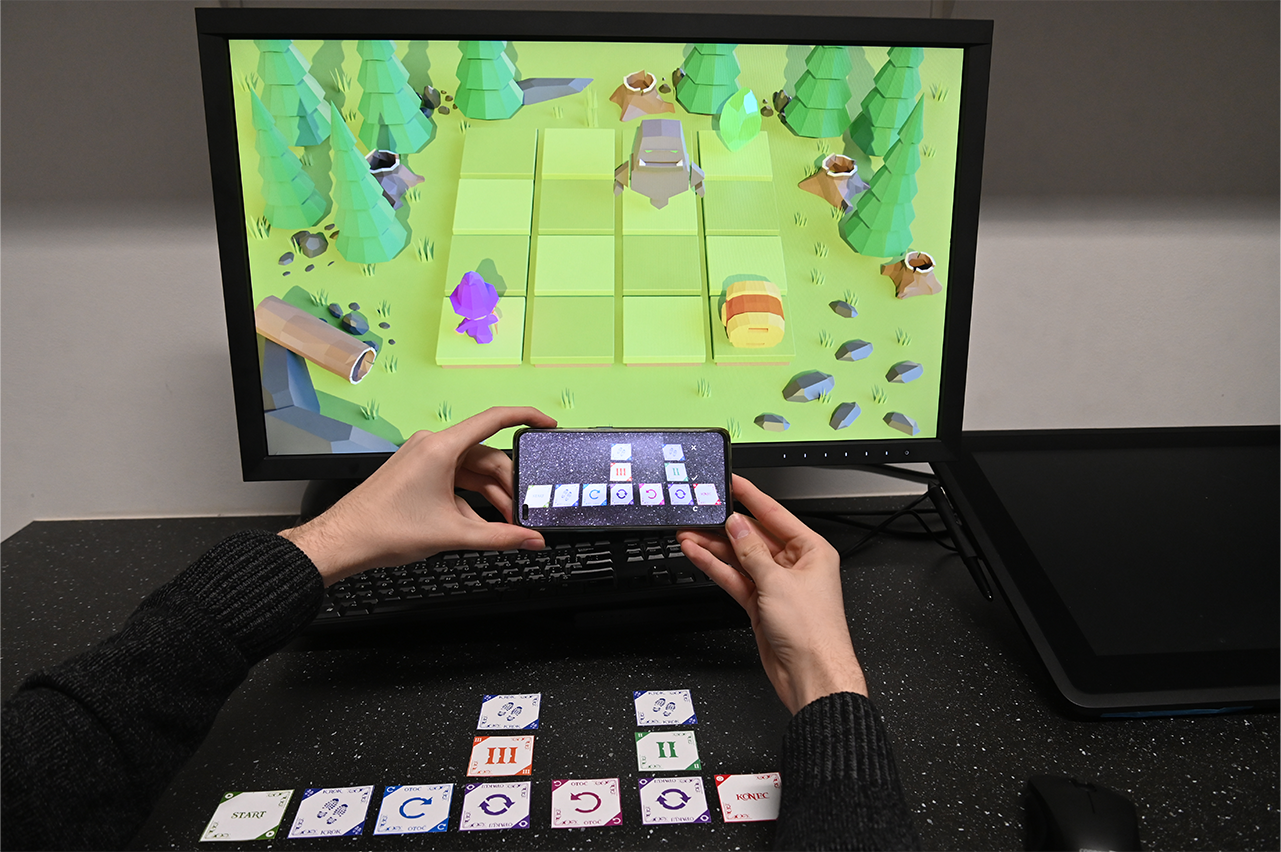
\includegraphics[width=0.6\textwidth]{img/pohled-hrace.png}
    \caption{Pohled hráče.}
    \label{fig:pohled-hrace}
\end{figure}


\chapter{Tipy k psaní}

Jak už jsem psal výše \LaTeX je dosti komplexní systém, který umožňuje psát velmi rozsáhlé text. Jeho autor Donald Knuth ho stvořil, aby mohl vydat jeho učebnici \emph{The Art of Computer Programming} a dodnes se je využíván pro sazbu skript, učebnic, článků či závěrečných prací. V této kapitole najdeš ukázky různých funkcí a balíčků \LaTeX u od těch nejzákladnějších až po složitější. Neznamená to nutně, že všechny musíš použít, ale když potřebuješ pomoct, tak je dobré mít oporu. 

Pokud s \LaTeX em úplně začínáš tak ti můžu doporučit přiručku \emph{Ne příliš stručný úvod do systému \LaTeX2e}~\cite{LaTeXprirucka}. Případně spoustu užitečných informací nalezneš na Wikibooks~\cite{wikibooksLaTeX}. Pokud narazíš na nějaký problém googli. Na internetu je spoustu fór, kde pravděpodobně už někdo podobný problém řešil. Asi nejvíce otho najdeš na stránce \emph{TeX - LaTeX Stackexchange} \cite{stackExchange}.


\section[Základy]{Základy: Text, obrázky, tabulky a citace} %%[Text, který bude v obsahu]{Text, který se vytiskne na stránce} Zkus měnit jednotlivé závorky a uvidíš :) 
Psaní v \LaTeX{u} není žádná věda, stačí psát normálně do zdrojového souboru. Pokud bys chtěl psát obrážky či číslovaný seznam, pak můžeš použít prostředí \texttt{itemize} či \texttt{enumerate}. Často je důležité používat nezlomitelnou mezeru. Tu uděláš pomocí \verb|~|~(tildy). Pokud budeš chtít psát uvozovky použij příkaz \texttt{uv}, pomocí něj se ti vytvoří uvozovky podle příslušného jazyka. V česku tedy ve formátu 99 66. Použití příkazu najdeš níže v textu.

Občas je zapotřebí \LaTeX{u} pomoct při rozdělování slov. To se udělá snadno vložením symbolů \verb|\-| mezi jednotlivé slabiky.

\subsection{Obrázky}

U obrázků je dobré používat vektorové formáty, pokud to jde. \LaTeX se nejvíc kamarádí s formátem PDF. Do známého PDFka lze z jiných vektorových formátů (ať už SVG či ESP) obrázky přenést snadno pomocí grafických programů, jako je třeba Inkscape. \LaTeX si rozhodně poradí i s tradičními formáty PNG a JPG, avšak tyto obrázky mohou zabírat více prostoru a při tisku se může projevit nižší rozlišení obrázků. Pokud chceš používat tyto obrázky, rozhodně měj na paměti, aby měli rozlišení alespoň 250 indálně 330 ppi.

Obrázky se vkládají do prostředí \texttt{figure}, při úpravě šířky je možné krom tradičních jednotek jako cm nebo mm použít také jako jednotku šířku stránky \texttt{textwidth} to se hodí zejména když chceš mít více podobrázků. 

U každého obrázku je důležité aby měl popisek, \texttt{caption}. Do popisku napiš, co na obrázku je, případně nějaký další popis, tak aby čtenář následně neměl sebemenší pochybnost. U obrázků co nejsou tvoje nezapomeň an citaci. Jinak by to totiž znamenalo, že jsi obrázek dělal ty sám, což není etické přivlastňovat si cizí díla. Popisek obrázku je věta, proto musí vždy končit tečkou.

\begin{figure}
    \centering %% příkaz, který ti obrázek zarovná na střed
    
\includegraphics[width=0.6\textwidth]{img/soc-logo.jpg} %% vložení samotného obrátku
    \caption{Logo SOČky \cite{socLogo}.} %% popisek obrázku, nezapomeň na citace!
    \label{fig:logoSOC} %% označení až budeš chtít na obrázek odkazovat
\end{figure}

Když chceš odkazovat na obrázek, stačí pak už jen napsat příkaz \texttt{ref} a do závorek napsat označení obrázku. Třeba logo SOČky, můžeš vidět na obrázku \ref{fig:logoSOC} \cite{socLogo}.

Pokud bys měl více podobrázků přichází do hry balíček \texttt{subcaption}. Pomocí něj lze vysázet i podobrázky. U podobrázků se popisek píše pouze jeden, dolů. Je v tomto připadě vhodné použít navíc hranaté závorky, do nichž se napíše kratší popisek, který se následně ukáže v seznamu obrázků.


\begin{figure}[h] \centering
    % \begin{subfigure}{0.63\textwidth} %%prostředí pro podobrázek {šířka podobrázku}
    %   \includegraphics[width=\textwidth]{imgs/vysledek_10} 
    %   \caption{} %% aby se ti vysázelo označení obrázku.
    % \end{subfigure}
    % \begin{subfigure}{0.63\textwidth}
    %   \includegraphics[width=\textwidth]{imgs/vysledek_20}
    %   \caption{}
    % \end{subfigure}
    \caption[Graf závislosti rotace DH PSF $\Delta\varphi$ na defokusaci objektivu $\Delta z$.]{Graf závislosti rotace DH PSF $\Delta\varphi$ na defokusaci objektivu $\Delta z$, (a) při použití objektivu Plan Fluor 10, (b) při použití objektivu Plan Fluor 20. Měřená data (žluté body) jsou lineárně proloženy (přerušovaná přímka). }
    \label{fig:rotace_grafy}
\end{figure}

Všimni si, že obrázky jsou naschvál široké. Je to proto, aby byly dobře čitelné. Také si všimni popisku grafů. Ačkoli nejspíš netušíš co je to DH PSF či defokusace objektivu mělo by ti být jasné, že je důležité přesně graf popsat. To znamená co je na vodorovné ose, co je na svislé ose. V jakých jednotkách veličiny jsou. Které body co znamenají, která křivka má jaký význam. Napsat samotné \uv{$\Delta \varphi$} je málo, vždy raději připoměň, co daná značka znamená.

\subsection{Tabulky}

U tabulek platí to stejné co u obrázků. Zarovnávají se na střed a nechávají se \uv{plavat} v textu. Tabulka narozdíl od textu, má popisek nahoře. U tabulky \ref{tab:ukazka} je použit balíček \texttt{booktabs}, pomocí kterého je celá tabulka naformátovaná.

Seznam jak obrázků tak tabulek je pak vytvořen pomocí příkazů \texttt{listoftables} a~\texttt{list\-of\-fig\-ures} na konci práce před literaturou.

\begin{table}[b]
    \caption{Tato tabulka slouží jako ukázka toho, jak mohou tabulky vypadat.} %% popisek se u tebaluky píše nad ní
    \label{tab:ukazka} %% označení pro pozdější odkazování se 
    \centering
        \begin{tabular}{lll}
            \toprule %% příkazy z balíčku booktabs
            záhlaví& této & tabulky\\
            \midrule
            obsah&tabulky& už\\
            není & oddělený &čarami\\
            \bottomrule
        \end{tabular}
\end{table}

\subsection{Literatura}

V \LaTeX{}u lze dělat seznam literatury dvěma způsoby. V této šabloně jsem použil ten, kdy se seznam literatury píše přímo do práce. Pro jeho vygenerování doporučuji použít některý z generátarů, jako jsou například Citace PRO \cite{citacePRO}. Pomocí citací lze vygenerovat přímo dokument, který se pak už jen překopíruje do textu a člověk nemusí nic zvýrazňovat. Dále lze využít Bibtex, který rozhodně do budoucna hodlám zaimplementovat do šablony, avšak jeho použití nemusí být tak přátelské k začátečníkům.

Pokud bys chtěl odkazovat na vícero zdrojů stačí je napsat vedle sebe oddělené čárkou \cite{LaTeXprirucka, citacePRO, Born2019}. Případně můžu odkaz na konkrétní stránku dát do hranatých závorek, viz \cite[str.~1]{Born2019}


\section[Pokročilejší tipy]{Pokročilejší tipy, které se mohou hodit}

\subsection{Rovnice}

Jak můžeš vidět tak rovnice lze psát jednak do textu a nebo pokud se jedná o nějakou důležitou nebo rozsáhlejší rovnici tak na samostatný řádek. Pokud je rovnice opravdu důležitá, tak je vhodné ji také číslovat. Pak se na ni můžeš dále odkazovat v textu.
\begin{equation}
    \vec{F} = m \vec{a}
    \label{eq:newton2}
\end{equation}
\dots Například podle druhého Newtonova zákona, rovnice (\ref{eq:newton2}) \dots Zároveň je vždy nutné vysvětlit co která veličina znamená. V tomto případě bych napsal, že v druhém Newtonově zákoně vektor síly $\vec F$ odpovídá součinu hmotnosti tělesa $m$ a jeho zrychlení $\vec a$. 

Věřím, že se sazbou matematiky ti pomůže tvůj školitel, případně mi můžeš napsat (mail je v úvodu). Jednotlivé funkcionality spolu se seznamem znaků nalezneš jednak v Ne příliš stručném úvodu~\cite{LaTeXprirucka} nebo na Wikibooks v sekcích \emph{Mathematics} a \emph{Advanced mathematics}~\cite{wikibooksLaTeX}.

\chapter{Když dokončuji práci}

Každou práci je dobré zkontrolovat, aby v ní nebyly pravopisné chyby, nebyla těžkopádně napsaná -- byla čtivá -- a neobsahovala žádný typografický nedostatek. Proto, když práci sepíšeš, nech ji chvilku odležet, třeba týden. Pak si ji po sobě znovu přečti. Hned uvidíš, kolik věcí bys napsal jinak případně kde tě bije do očí jaká chyba. Dej práci přečíst také svému školiteli a případně češtináři. Zajistíš tak, že bude obsahovat méně chyb.

Pak můžeš práci vytisknout a hurá do soutěže.

\chapter{Závěr}

Věřím, že jsem ti spolu se šablonou poskytl několik tipů, jak napsat práci. Ať už jde o úplné začátky s \LaTeX{}em. Či ukázku toho, co vše s ním zvládneš. Pokud bys měl k šabloně libovolné dotazy, rouhodně se na mě obrať. \LaTeX tvé práci dodá určitou krásu, tak doufám, že ti dodá sebevědomí a uspěješ při souteži. A i kdyby ne vzpomeň si, kolik ses toho musel naučit a hned uvidíš o jaký kus ses posunul.